\chapter{Code Block Generation} \label{chap:codeBlock}
Jupyter Notebooks are valued for their effectiveness in writing and revising 
code for data research. They allow code to be written in discrete blocks (or 
``cells"), which can be executed separately, as opposed to writing and running 
a whole program \cite{jupyterNotebookUsage}. This allows for a mix of content 
types, including equations, figures, and graphs, with code to better present 
information. 

In Chapter~\ref{chap:nbprinter}, we cover two types of metadata in Jupyter 
Notebooks: one type is necessary for forming the notebook, while the other is 
required to create cells for the contents. We explain how to generate the 
metadata and create a Markdown cell. When generating the SRS, we do not need to 
worry about generating code blocks since the SRS does not include any code. 
However, when creating lesson plans (or user manuals), we likely want to 
integrate real examples that involve code. As we are now combining text and 
code in a document, we need to address the following questions before 
generating the right type of cell: i) what type of cell should we use, Markdown 
or code? and ii) how do we know when to end a cell and start a new one? That 
is, how do we determine where to split the contents into cells?
 
To begin, we need to consider the conceptual definition of a cell in Jupyter 
Notebooks. A cell is essentially a standalone unit of information or code that 
can be executed independently. In other words, it is a unit of content within 
the notebook \cite{cellsseparation}. A cell can contain either text or code and 
can span multiple lines. Understanding the relationship between cells and their 
contents is crucial for implementing an effective splitting strategy. By 
identifying natural boundaries within the text or code and recognizing the unit 
of the contents, we can determine where to split the contents into cells.

In this chapter, we will discuss different approaches and implementations for 
splitting the contents and generating the appropriate type of cells.

\section{Unit of Contents}
To organize the contents of a lesson plan, we use two different approaches: by 
sections and by content types. We will discuss the advantages and disadvantages 
of these approaches.

\subsection{Section-level}
When considering what would be the appropriate unit of content for splitting, 
one might first think of paragraphs or sections. In the source language of 
Drasil, since a document is made up of sections (as seen in 
Code~\ref{code:drasil-lang-document}), it may appear reasonable to split these 
sections into individual cells. However, the nested structure of Drasil 
documents, where each \texttt{Section} is composed of a list of 
\texttt{Contents} and \texttt{Section}s (as demonstrated in 
Code~\ref{code:section}), does not align well with the sequential flow of a 
Jupyter Notebook. To address this issue, we flatten the structure of the Drasil 
document by making each section and subsection an independent 
\texttt{Section}. 

We have updated the definition of \texttt{Section} data type 
(Code~\ref{code:newoldsection}). In the new definition (line 9-16), the 
\texttt{Depth} attribute is used to keep track of the level of each section, 
with 0 indicating the parent section, 1 indicating the subsection, 2 indicating 
the sub-subsection, and so on. Furthermore, we have replaced the 
\texttt{SecCons} attribute, which previously represented both sections and 
contents, with a new attribute that allows each section to only have contents. 

For example, Code~\ref{code:IntroSec} defines the Introduction 
section, where 
the original nested structure (lines 1-12) comprises a list of subsections, 
while in the flattened version (lines 13-21), each subsection is self-contained 
and has its own type. Code~\ref{code:DocSection} further illustrates that each 
section is independent after the changes.

\begin{listing}[h]
	\caption{Nested and Flattened Section Comparison}
	\label{code:newoldsection}
	\begin{lstlisting}[language=haskell1]
		-- Nested Structure
		data Section = Section
							   { tle  :: Title
							   , cons :: [SecCons]
							   , _lab :: Reference
							   }
		makeLenses ''Section
		
		-- Flattened Structure
		data Section = Section 
							  { dep  :: Depth 
							  , tle  :: Title
							  , cons :: [Contents]
							  , _lab :: Reference
							  }
		makeLenses ''Section
	\end{lstlisting}
\end{listing}

\begin{listing}[h]
	\caption{Nested and Flattened Introduction Comparison}
	\label{code:IntroSec}
	\begin{lstlisting}[language=haskell1]
		-- Nested Structure
		-- | Introduction section. Contents are top level 
		-- followed by a list of subsections.
		data IntroSec = IntroProg Sentence Sentence [IntroSub]
		
		-- | Introduction subsections.
		data IntroSub where
			IPurpose :: [Sentence] -> IntroSub
			IScope   :: Sentence -> IntroSub
			IChar    :: [Sentence] -> [Sentence] -> [Sentence] -> IntroSub
			IOrgSec  :: Sentence -> CI -> Section -> Sentence -> IntroSub
	
		-- Flattened Structure
		-- | Introduction section.
		data IntroSec = IntroProg Sentence Sentence
	
		-- | Introduction subsections.
		newtype IPurpose = IPurposeProg [Sentence] 
		newtype IScope = IScopeProg Sentence 
		data IChar = ICharProg [Sentence] [Sentence] [Sentence]
		data IOrgSec = IOrgProg Sentence CI Section Sentence
	\end{lstlisting}
\end{listing}

\begin{listing}[h]
	\caption{Pseudocode for Definition of DocSection}
	\label{code:DocSection}
	\begin{lstlisting}[language=haskell1]
		-- Nested Structure
		data DocSection = TableOfContents
										| RefSec RefSec
										| IntroSec IntroSec
										| StkhldrSec StkhldrSec
										...
		
		-- Flatten Structure
		data DocSection = TableOfContents TableOfContents
										| RefSec RefSec
										| TUnits TUnits
										| TSymb TSymb
										| TAandA TAandA
										| IntroSec IntroSec
										| IPurposeSub IPurposeSub
										| IScopeSub IScopeSub
										| ICharSub ICharSub
										| IOrgSub IOrgSub
										...
		
	\end{lstlisting}
\end{listing}
 
While flattening the structure of a document can allow for it to be split into 
individual cells by sections, there are limitations to this approach. Splitting 
the contents at the section level might not always be the most effective 
approach. It's possible that certain sections might be too long to fit 
comfortably in a single cell. Moreover, when working with documents that 
combine text and code (such as lesson plans), section-level splitting may not 
be appropriate due to the different types of cells needed for text and code. 
Therefore, a better approach is needed, as presented in the next section.

\subsection{LayoutObj-level}
In Jupyter Notebook, a cell can be seen as a self-contained unit of 
information, and it can contain multiple types of content, such as text, code, 
and figures. To determine the appropriate unit of content for splitting, we 
need to consider the content itself and what makes sense in terms of its 
structure and organization.  Although a cell might not always be the most 
appropriate unit of content for splitting, it is somehow the lowest level of 
``display content" that conveys a coherent piece of information 
\cite{cellsseparation}. Therefore, splitting the content based on logical units 
of information might be a more effective approach rather than using sections as 
the sole criterion. 

In previous chapters, we discussed how Drasil handles different types of 
content through the use of the \texttt{RawContent} data type, which includes 
paragraphs, figures, equations, and other content types 
(Code~\ref{code:RawContent}). A Drasil \texttt{Section} can consist of a list 
of \texttt{RawContent}, allowing for the inclusion of different types of 
content within a single section. Additionally, as we saw in 
Chapter~\ref{chap:nbprinter}, the document is printed in a specific document 
language using \texttt{LayoutObj}, which is derived from \texttt{RawContent}. 
Because each content type is handled explicitly by \texttt{LayoutObj}, we can 
take advantage of this and split each type of content into its own cell.

To implement this approach, we first need to ensure that each layout object 
is generated independently and is not nested with other layout objects. In 
Chapter~\ref{chap:nbprinter}, we discussed how \texttt{RawContent} is 
translated to a printable \texttt{LayoutObj}. The \texttt{printLO} function in 
Code~\ref{code:LayoutObj} demonstrates how the printer renders each content 
type into a notebook format. However, the current format of \texttt{LayourObj} 
is designed for the SRS and may not be suitable for lesson plans. For instance, 
the \texttt{HDiv}\footnote{The \texttt{HDiv} is a printable layout object 
that's designed to create HTML documents. The main purpose is to wrap contents 
in the $<$div$>$ tag.} type wraps sections and creates an HTML $<$div$>$ tag, 
and even an equation block is translated into the \texttt{HDiv}, 
as seen in Code~\ref{code:EqnblocktoTex]}. Moreover, the \texttt{Definition} 
type is designed for the definition or model defined in the SRS and may not be 
required for lesson plans. To better accommodate lesson plan content types, we 
may need to create a new \texttt{LayoutObj} in the future when we have a 
better understanding of the lesson plan structure.

Currently, we are using the existing \texttt{LayoutObj} to translate our 
lesson plan contents into printable layout object. Since these contents are not 
code and should be in Markdown, we print each required content type 
independently into a Markdown cell. To accomplish this, we use the 
\texttt{markdownCell} function from Code~\ref{code:markdownCell}. This function 
generates the necessary metadata and creates the Markdown cell for each layout 
object, which is our unit of content. 

Code~\ref{code:printLO'} illustrates how each content type is rendered in 
notebook format in a Markdown cell. For layout objects that are not needed in 
lesson plans, we make them empty. We also separate equation blocks from 
\texttt{HDiv} with the equation tag to have more control over the structure.

\begin{listing}[h!]
	\caption{Source Code for printLO'}
	\label{code:printLO'}
	\begin{lstlisting}[language=haskell1, basicstyle=\small\ttfamily]
		-- printLO' is used for generating lesson plans
		printLO' :: LayoutObj -> Doc
		printLO' (HDiv ["equation"] layObs _) = markdownCell $ 
			vcat (map printLO' layObs)
		printLO' (Header n contents l) = markdownCell $ nbformat 
			(h (n + 1) <> pSpec contents) $$ refID (pSpec l)
		printLO' (Cell layObs) = vcat (map printLO' layObs)
		printLO' HDiv {} = empty
		printLO' (Paragraph contents) = markdownCell $ nbformat 
			(stripnewLine (show(pSpec contents)))
		printLO' (EqnBlock contents) = nbformat mathEqn
			where
				toMathHelper (PL g) = PL (\_ -> g Math)
				mjDelimDisp d = text "$$" <> stripnewLine (show d) <> text "$$" 
				mathEqn = mjDelimDisp $ printMath $ toMathHelper $ 
					TeX.spec contents
		printLO' (Table _ rows r _ _) = markdownCell $ 
			makeTable rows (pSpec r)
		printLO' (Definition dt ssPs l) = empty
		printLO' (List t) = markdownCell $ makeList t False
		printLO' (Figure r c f wp) = markdownCell $ makeFigure 
			(pSpec r) (pSpec c) (text f) wp
		printLO' (Bib bib) = markdownCell $ makeBib bib
		printLO' Graph{} = empty
	\end{lstlisting}
\end{listing}

As splitting contents by their types rather than sections makes more sense and 
better satisfies our needs, we can keep the document structure nested. Also, as 
the structure of our lesson plans is already linear, we can achieve the goal of 
breaking contents into smaller units by adopting only the second approach.

\section{Code Block}
We split contents with our content types for various reasons, including the 
need to differentiate between Markdown contents and code to generate the 
appropriate type of cell and to specifically deal with each type of content. 
To better manage and generate code in Jupyter Notebook with Drasil, we 
introduce a new content type called \texttt{CodeBlock}. Like other content 
types, a \texttt{CodeBlock} is defined within \texttt{RawContent}, which 
requires a \texttt{CodeExpr} as shown in Code~\ref{code:newRawContent}.

\begin{listing}[h!]
	\caption{Source Code for the New Definition of RawContent}
	\label{code:newRawContent}
	\begin{lstlisting}[language=haskell1]
		-- | Types of layout objects we deal with explicitly.
		data RawContent =
		Table [Sentence] [[Sentence]] Title Bool
		| Paragraph Sentence                       
		| EqnBlock ModelExpr                      
		| DerivBlock Sentence [RawContent]        
		| Enumeration ListType                    
		| Defini DType [(Identifier, [Contents])] 
		| Figure Lbl Filepath MaxWidthPercent     
		| Bib BibRef                              
		| Graph [(Sentence, Sentence)] (Maybe Width) (Maybe Height) Lbl
		| CodeBlock CodeExpr   
	\end{lstlisting}
\end{listing}

\texttt{CodeExpr} is a language (pre-existing in Drasil) that allows us to 
define code expressions. It shares similarities with \texttt{Expr} functions, 
constructors, and operators, but is tailored specifically for generating code. 
We utilize this data type to define and encode the expressions for our Jupyter 
Notebook code. 

The process of handling code blocks and printing the code within a code cell 
is similar to how we handle other Markdown contents, as discussed in the 
previous chapters. However, the conversion is unique to the \texttt{CodeBlock} 
type. For instance, to encode the code, we can use the \texttt{unlbldCode} 
(Code~\ref{code:unlbldCode}) function, which converts a \texttt{CodeExpr} to 
\texttt{Contents}.

\begin{listing}[h!]
	\caption{Source Code for Rendering CodeBlock to LayoutObj}
	\label{code:unlbldCode}
	\begin{lstlisting}[language=haskell1]
		-- | Unlabelled code expression
		unlbldCode :: CodeExpr -> Contents
		unlbldCode c = UlC $ ulcc $ CodeBlock c
	\end{lstlisting}
\end{listing}

After encoding the code expressions in Drasil, the printer then converts the 
code blocks into printable layout objects, as defined in 
Code~\ref{code:newLayoutObj}, using the methods in 
Code~\ref{code:codeBlocktoLayObj}. The resulting content, which is a 
\texttt{RawContent}, is translated into a printable object, a 
\texttt{LayoutObj}, before being processed by the document language printer. 

\begin{listing}[h!]
	\caption{Source Code for the New Definition of LayoutObj}
	\label{code:newLayoutObj}
	\begin{lstlisting}[language=haskell1]
		data LayoutObj = 
				Table Tags [[Spec]] Label Bool Caption                          
			| Header Depth Title Label                                       
			| Paragraph Contents                                              
			| EqnBlock Contents                                               
			| Definition DType [(String,[LayoutObj])] Label                   
			| List ListType                                                   
			| Figure Label Caption Filepath MaxWidthPercent                  
			| Graph [(Spec, Spec)] (Maybe Width) (Maybe Height) Caption Label 
			| CodeBlock Contents  
			| HDiv Tags [LayoutObj] Label                                    
			| Cell [LayoutObj] 
			| Bib BibRef     
	\end{lstlisting}
\end{listing}

\begin{listing}[h!]
	\caption{Source Code for Rendering CodeBlock to LayoutObj}
	\label{code:codeBlocktoLayObj}
	\begin{lstlisting}[language=haskell1]
		-- | Helper that translates 'LabelledContent's to a 
		-- printable representation of 'LayoutObj'.
		layLabelled sm (LblC _ (CodeBlock c)) = T.CodeBlock 
		(P.E (codeExpr c sm))
		-- | Helper that translates 'RawContent's to a 
		-- printable representation of 'LayoutObj'.
		layUnlabelled sm (CodeBlock c) = T.CodeBlock (P.E (codeExpr c sm))
	\end{lstlisting}
\end{listing}

Generating a code cell in Jupyter Notebook requires metadata, similar to 
generating a markdown cell. However, since the metadata is identical across 
code cells, the \texttt{codeCell} function generates the required metadata and 
creates a code cell for the given code, which is the `contents' in 
Code~\ref{code:codeBlocktoJSON}. This constructor eliminates the need for 
redundant metadata specification and provides a convenient way to generate code 
cells in Jupyter Notebook.

\begin{listing}[h!]
	\caption{Source Code for Generating a CodeBlock}
	\label{code:codeBlock}
	\begin{lstlisting}[language=haskell1]		
		-- | Helper for generate a Code cell
		codeCell :: Doc -> Doc
		codeCell c = codeB <> c <> codeE
		
		codeB, codeE :: Doc
		codeB = text "  {\n   \"cell_type\": \"code\",\n   
			\"execution_count\": null,\n   \"metadata\": 
			{},\n   \"outputs\": [],\n   \"source\": [" 
		codeE  = text "\n   ]\n  },"
		\end{lstlisting}
\end{listing}

Finally, the JSON printer takes the printable layout object of the code block, 
prints the code, converts it to the notebook format, and generates a code cell, 
as demonstrated in Code~\ref{code:codeBlocktoJSON}.

\begin{listing}[h!]
	\caption{Source Code for Rendering CodeBlock into JSON}
	\label{code:codeBlocktoJSON}
	\begin{lstlisting}[language=haskell1]
		-- | Helper for rendering CodeBlock into JSON
		printLO' (CodeBlock contents) = codeCell $ nbformat $ cSpec contents
	\end{lstlisting}
\end{listing}

The benefits of using Jupyter Notebook lie in its ability to allow users to 
write a portion of code and combine it with text. We have discussed various 
approaches to split the contents and generate the appropriate types of cell. 
The Projectile Motion Lesson generated by Drasil (an snapshot of the example 
chapter is shown in Figure~\ref{fig:example_drasil}), demonstrates that we are 
able to mix text and code and generate the appropriate cell types in Jupyter 
Notebook with Drasil. The source code for encoding this example can be found in 
Code~\ref{code:encodeExample}. In comparison, Figure~\ref{fig:example_manual} 
shows the same part created manually.

\begin{figure}[h!]
	\caption{Snapshot of Example Chapter Generated using Drasil}
	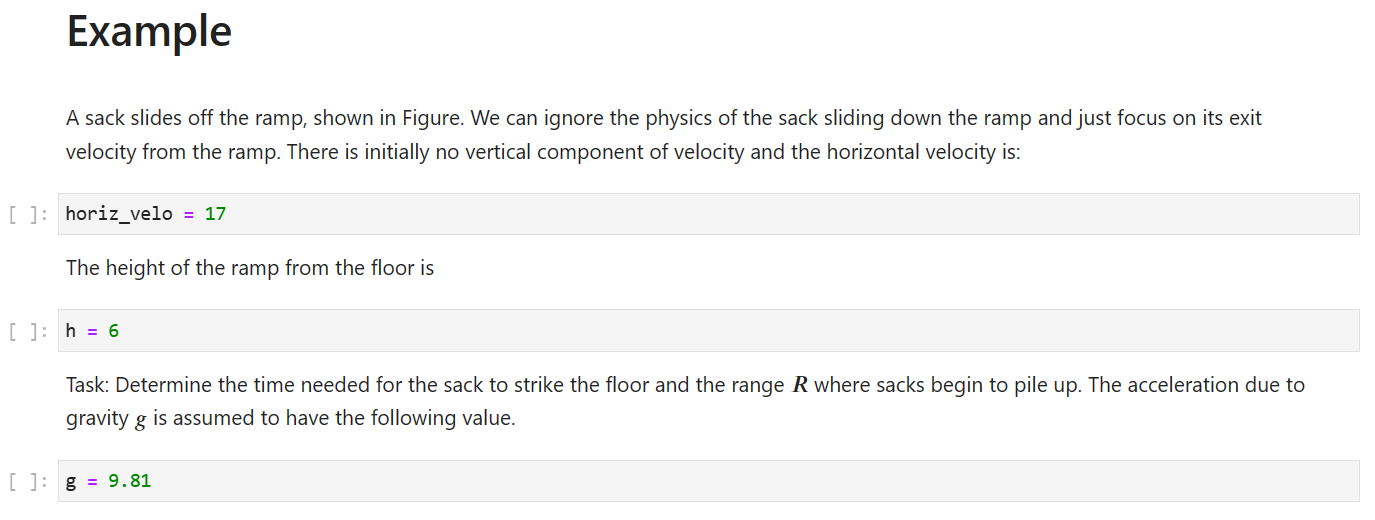
\includegraphics[width=1\textwidth]{figures/example_drasil.png}
	\label{fig:example_drasil}
\end{figure}

\begin{figure}[h!]
	\caption{Snapshot of Example Chapter Created Manually}
	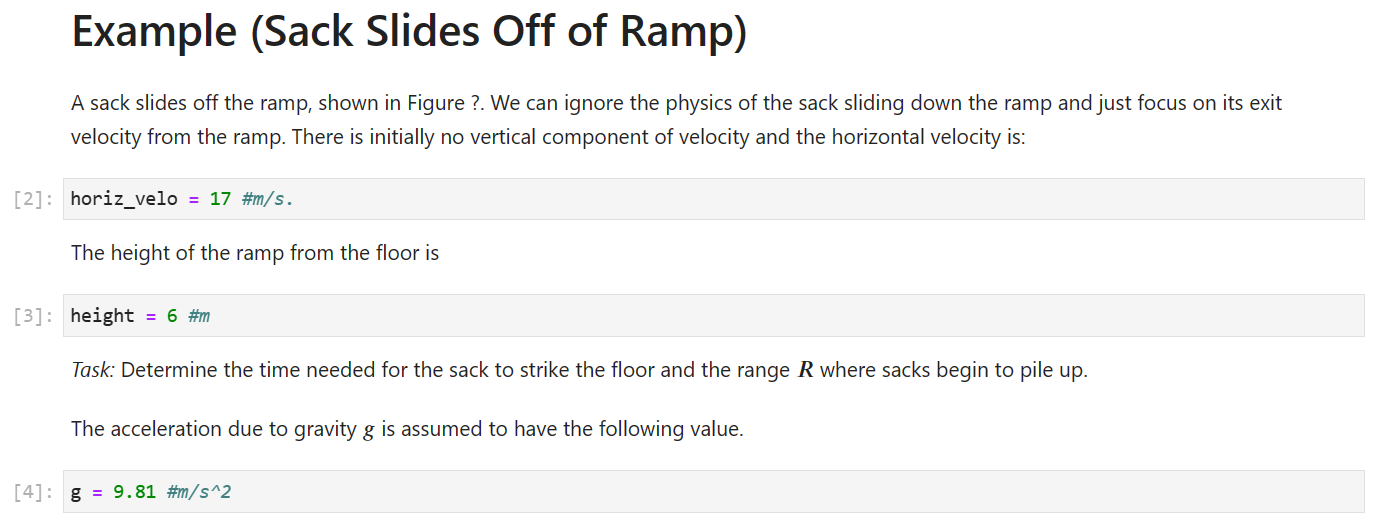
\includegraphics[width=1\textwidth]{figures/example_manual.png}
	\label{fig:example_manual}
\end{figure}

\begin{listing}[h!]
	\caption{Source Code for Encoding Example Chapter}
	\label{code:encodeExample}
	\begin{lstlisting}[language=haskell1]
	exampleContent :: [Contents]
	exampleContent = [exampleContextP1, codeC1, 
		exampleContextP2, codeC2, exampleContextP3, codeC3]
		
	exampleContextP1, exampleContextP2, exampleContextP3 :: Contents
	exampleContextP1 = foldlSP_ [S "A sack slides off the
		ramp, shown in Figure.", S "We can ignore the physics 
		of the sack sliding down the ramp and just focus on 
		its exit", phrase velocity +:+. S "from the ramp",
		S "There is initially no vertical component of", 
		phrase velocity `S.andThe` S "horizontal", 
		phrase velocity, S "is:"]
	exampleContextP2 = foldlSP_ [S "The", phrase height 
		`S.ofThe` S "ramp from the floor is"]
	exampleContextP3 = foldlSP_ [S "Task: Determine the", 
		phrase time, S "needed for the sack to strike the 
		floor and the range", P cR +:+. S "where sacks begin 
		to pile up", S "The", phrase acceleration, S "due to", 
		phrase gravity, P lG +:+. S "is assumed to have the 
		following value"]
		
	codeC1, codeC2, codeC3 :: Contents
	codeC1 = unlbldCode (sy horiz_velo $= exactDbl 17)
	codeC2 = unlbldCode (sy QP.height $= exactDbl 6)
	codeC3 = unlbldCode (sy QP.gravitationalAccel $= dbl 9.81)
	\end{lstlisting}
\end{listing}